\documentclass[10pt,a4paper]{article}
\usepackage[utf8]{inputenc}
\usepackage{amsmath}
\usepackage{amsfonts}
\usepackage{amssymb}
\usepackage{graphicx}
\usepackage{enumerate}
\begin{document}

\section{Set Theory}

To demystify mathematics consider
\begin{enumerate}[(i)]
\item What is a theorem?
\item What is a proof?
\end{enumerate}
What if we don't know the answer?

To begin we need
\begin{enumerate}[(a)]
\item an example(s)
\item a nearly related concept
\end{enumerate}


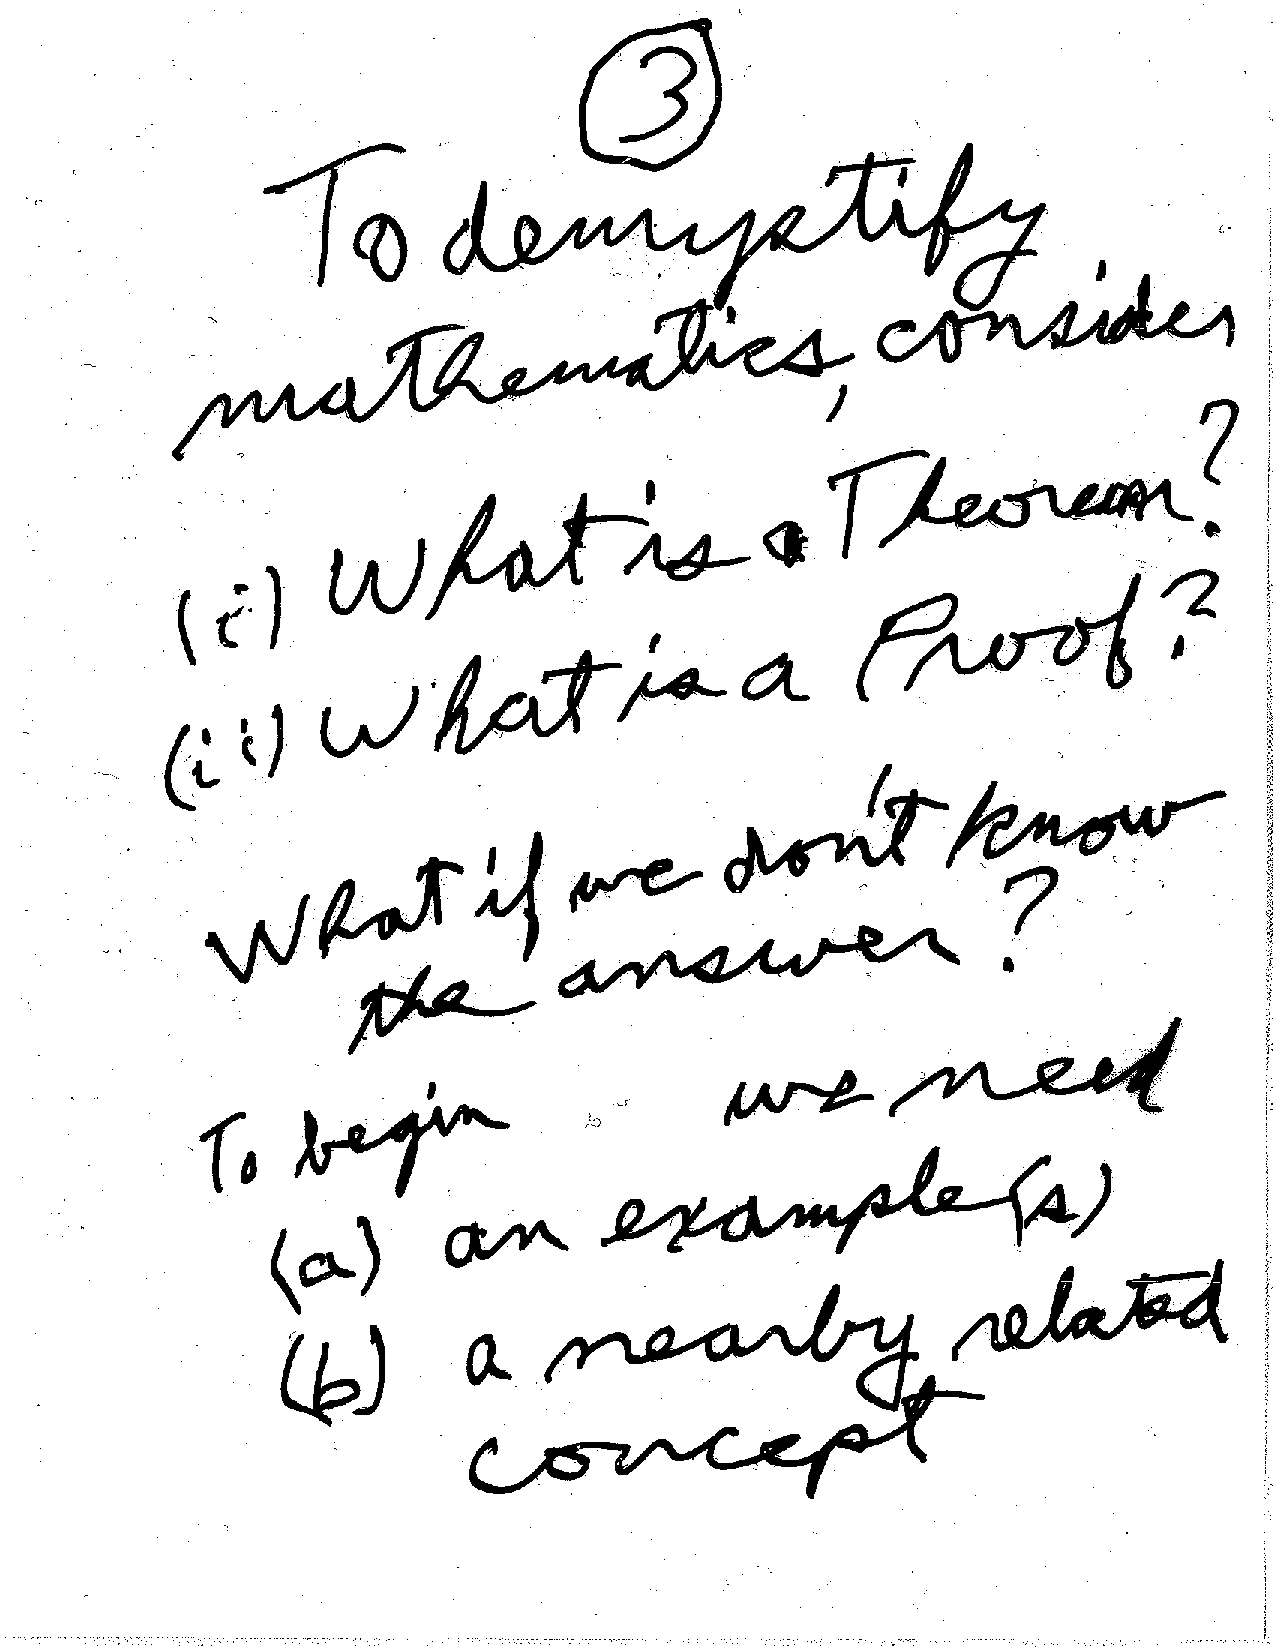
\includegraphics[scale=.5]{Pages/ST_3}

\newpage

Related Concept: Greek Syllogism

\underline{example:}
\begin{enumerate}
\item All men are mortal.
\item Socrates is a man.
\item Therefore, Socrates must die. 
\end{enumerate}

To analyze, recast in set theoretic terms via Venn Diagram.

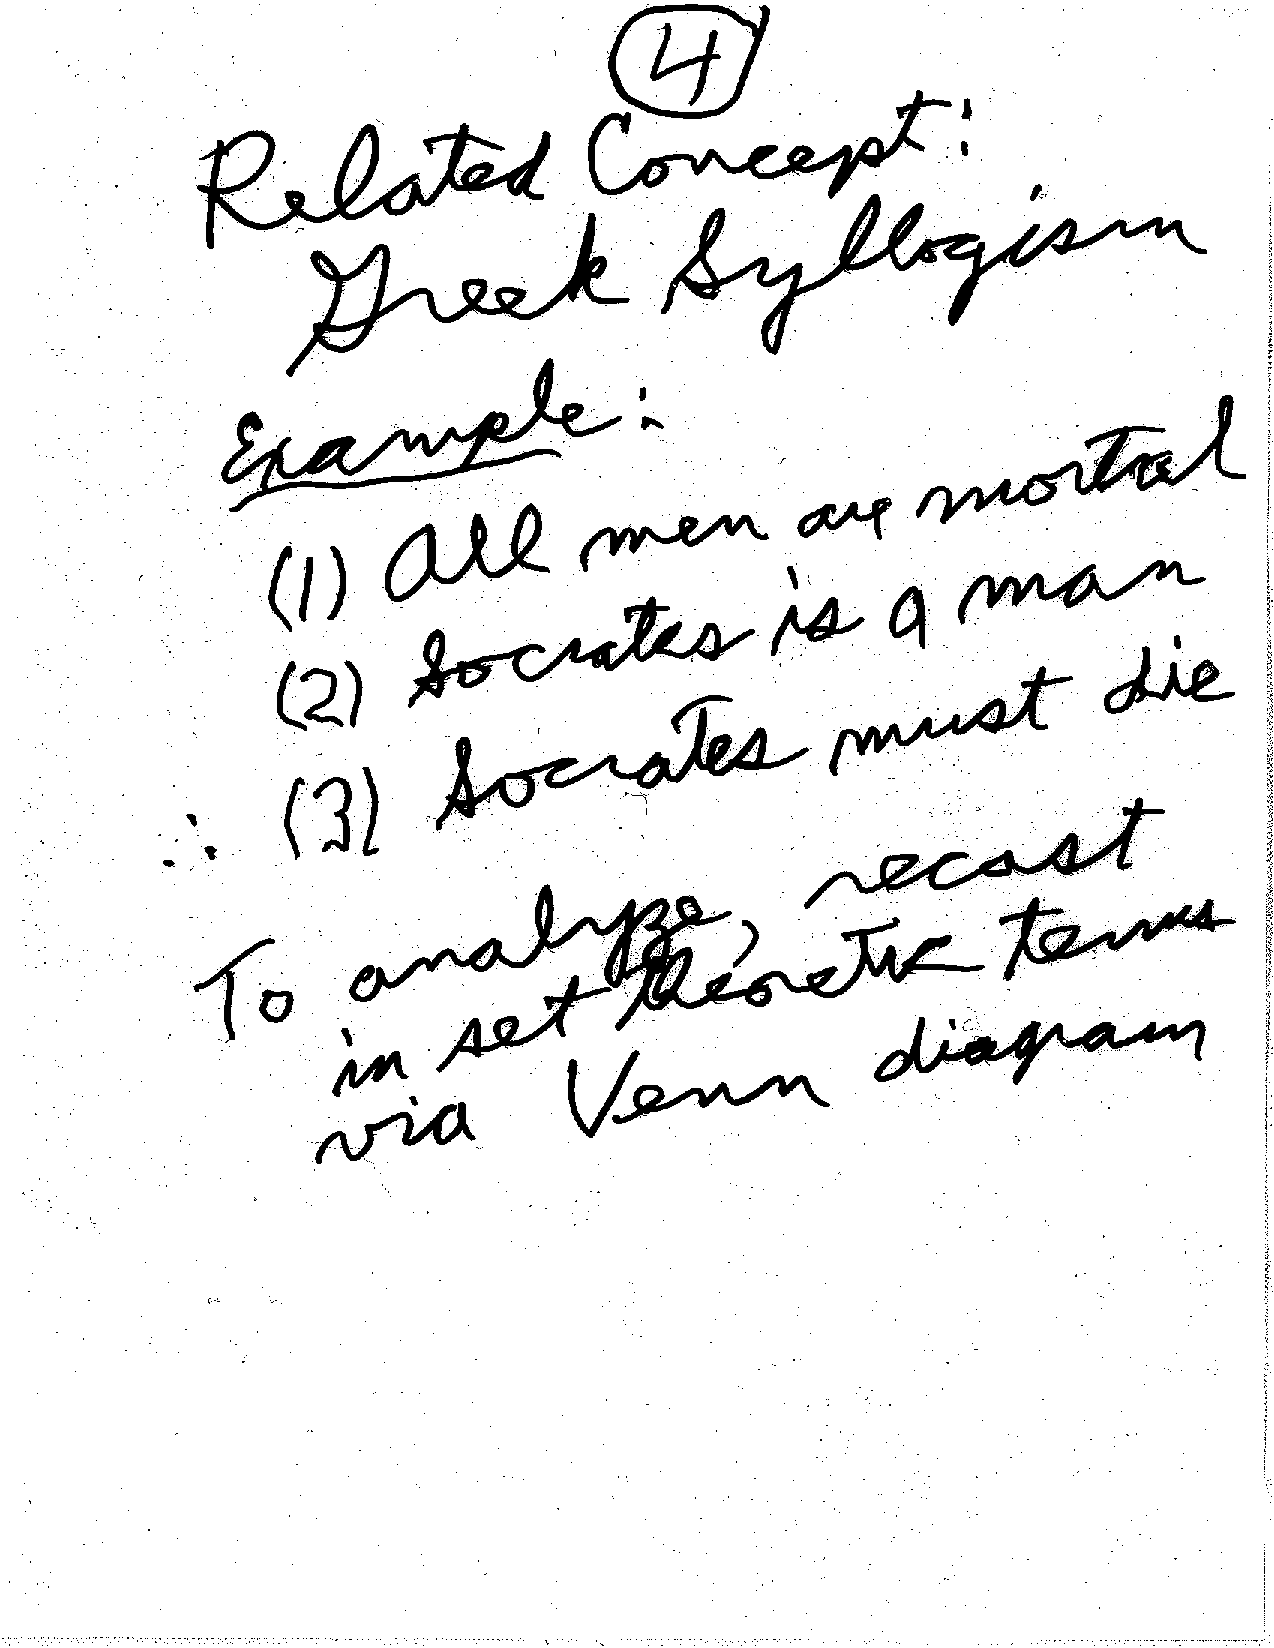
\includegraphics[scale=.5]{Pages/ST_4}

\newpage

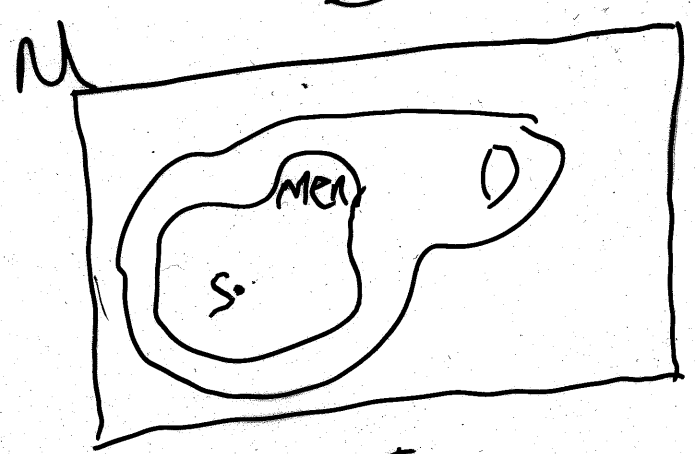
\includegraphics[scale=.2]{Pages/ST_5_im1}

$S$: Socrates\\
$M$: Set of Men\\
$D$: Things that will die\\
$\mathcal{U}$: Things on Earth

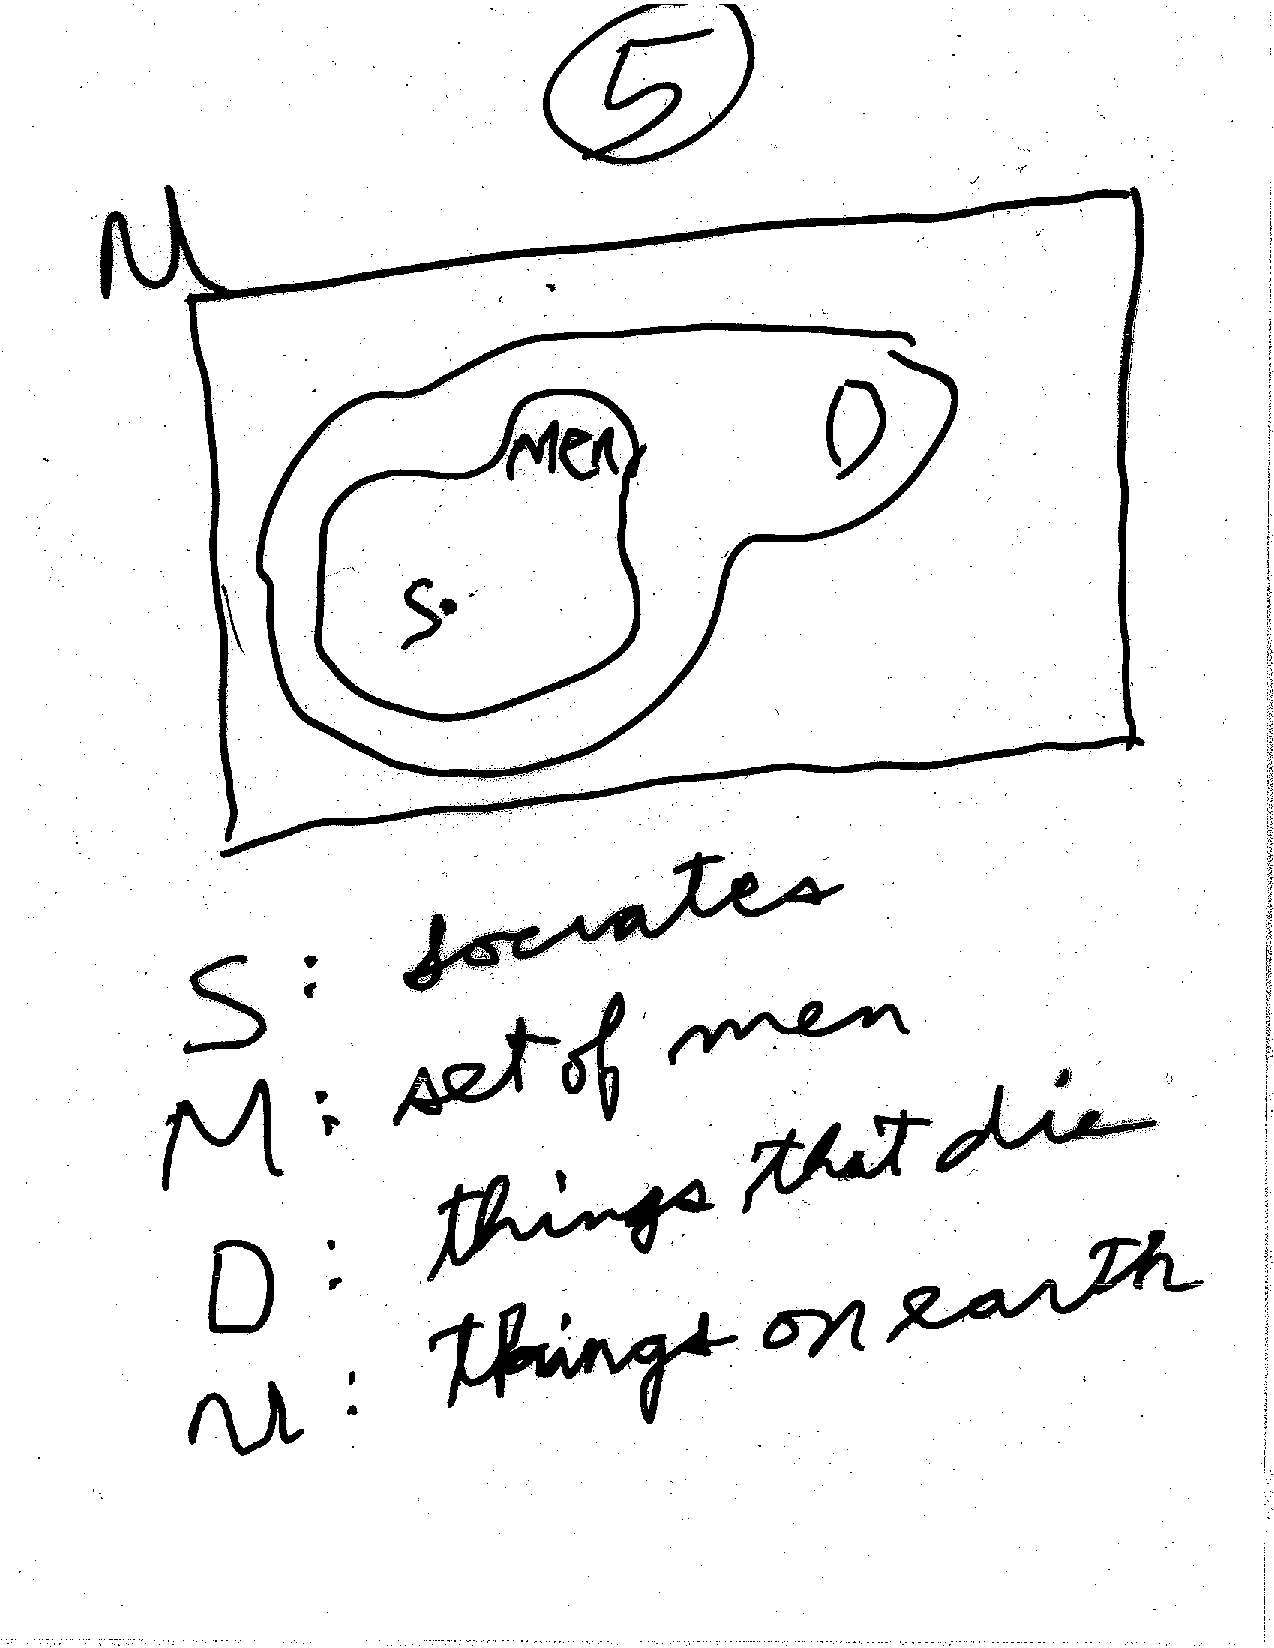
\includegraphics[scale=.5]{Pages/ST_5} 



%Zack: Pages 6,7,8,19,20

%Jack: 21, 9, 10, 11

%Koka: Pages 13, 13A, 22 ,22A, 22B


\section{Generate $\mathbb{N}$}


%Ruth: Pages L4A-L4G




\section{From $\mathbb{Z}$ to $\mathbb{R}$ via ordering}
%Jazz: ZR1-ZR5

%Kyler: ZR6 - ZR10

%Preethika: ZR11-ZR14


\section{Sequence and Limits}

%Aaron: First 2 pages and 48-50

%Hamza: 51-52B

\section{Limit and Convergence}

%Joe: 50-51

%Quinten: 52-53

%Farishta: 53A-54A

\section{Infinite Series}

%Sukhreet: IS1 - IS 7

%Matthew: IS8 - IS15

%Will: IS16 - IS23

\newpage %16

\begin{center}

{Infinite Series 16}

\end{center}

(ie) Suppose $r_{*} > 1$

Take $1 < \lambda < r_{*}$

$\exists N:N>N$

$=> |{\frac{{^a}n+1}{an}}| = \lambda$

We assume this means

$|a_{n}| > O$ for $n \geq N$

ntense $|{^a}N+K|\geq \lambda {^k}$

for $k\geq1$ so that

$|{^a}N+K|->\infty$ and $N+K-$

goes to infinity

this $\Sigma$an diverges

\begin{center}

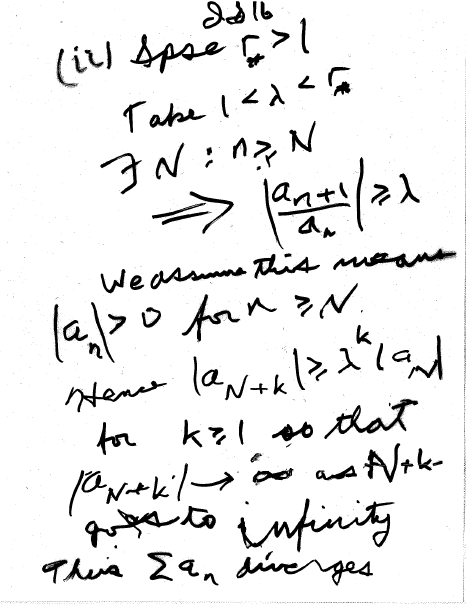
\includegraphics[scale=1]{Pages/IS_16}

\end{center}

\newpage %17

\begin{center}

Infinite Series 17

\end{center}

Case 1

\begin{center}

$(iii) a_{n} = n$ $r_{what} = r^{what} = 1$

$\Sigma a_{n} = \infty$ 

\end{center}

Case 2

\begin{center}

$a_{n} = \frac{1}{n^{2}}$ $r_{*} = r^{*} = 1$

yet $\Sigma a_{n} < \infty$

Pf: $= \infty \Sigma n=1 \frac{1}{n{2}} \leq \infty \Sigma n=1 \frac{2}{n(n+1)}$

\end{center}

$=lim 2 N n=1 \Sigma ({\frac{1}{n}}-{\frac{1}{n+1}})$

$=lim {\underset{\text{$N\Rightarrow \infty$}}{lim 2}}(1-\frac{1}{N+1})$

$=2<\infty$

Hence a series for which $r_{*}\leq 1\leq r^{*}$ is either common div?
\begin{center}

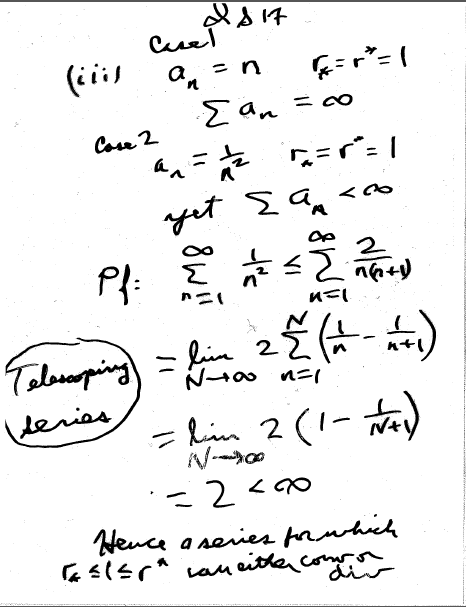
\includegraphics[scale=.7]{Pages/IS_17}

\end{center}

\newpage %18

\begin{center}

Infinite Series 18

\end{center}

A refinement of the ratio teat, the Root Test does not 
require that evenly excessive ratio is "well-behaved", but merely that some p-what preponderance are.
{\underline {Then}} let r $=$ ${\underset{\text{$N\Rightarrow \infty$}}{lim}}|a_{n}|^\frac{1}{n}$

(i) if $r<1$ the something corns absolutely

(ii) if $r>1$ the something diverges

(iii) if $r=1$ the test is inconclusive

\begin{center}

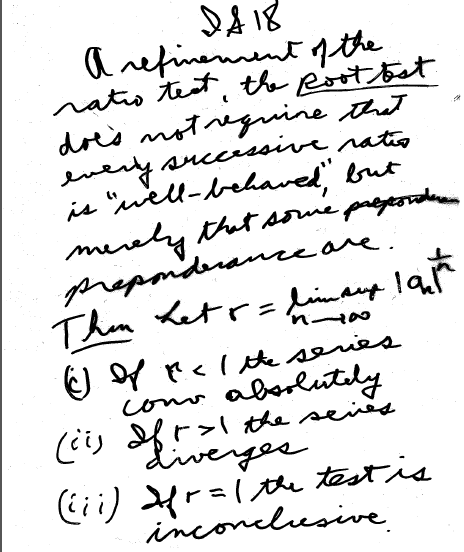
\includegraphics[scale=.7]{Pages/IS_18}

\end{center}

\newpage %19

\begin{center}

Infinite Series 19

\end{center}

Pf: (i) Suppose $r<1$ and take any $r<\lambda <1$

$\exists N: n \geq N => |a_{n}|^{\frac{1}{n}} \leq \lambda$

ntense $|a_{n}| \leq what^{n}$

By the comparison test $\Sigma a_{n}$ comes ahead.

(ii) Suppose $r>1$ and the $1<\lambda<r$

For {\underline {any}} $N < \infty$

$\exists n > N : |a_{n}|^{\frac{1}{n}} \geq what$

ntence lim says $|a_{n}| = \infty$

$n->\infty$

$\Sigma a_{n} diveges$

(iii) if $r=1$, test fail

\begin{center}

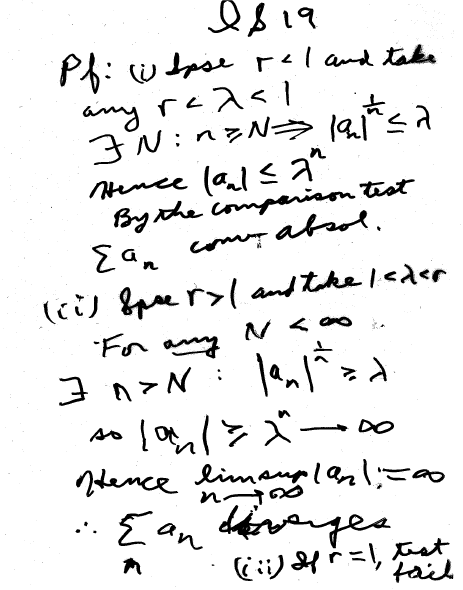
\includegraphics[scale=.7]{Pages/IS_19}

\end{center}

\newpage %20

\begin{center}

Infinite Series 20

{\underline {Power Series}}

\end{center}

Let $f(x) = \infty \Sigma$ $n=0$ $a_{n}x^{n}$

Let $R = {\frac{1}{lim}}|a_n|^{\frac{1}{n}}$

Then

(i) series comes absol for $o\leq |x|<R$

(ii) series div for ${x}>R$

(iii) at $x=R$ we may have common div

$O\leq R\leq \infty$ . R is called the radius of com of the power series.
\begin{center}

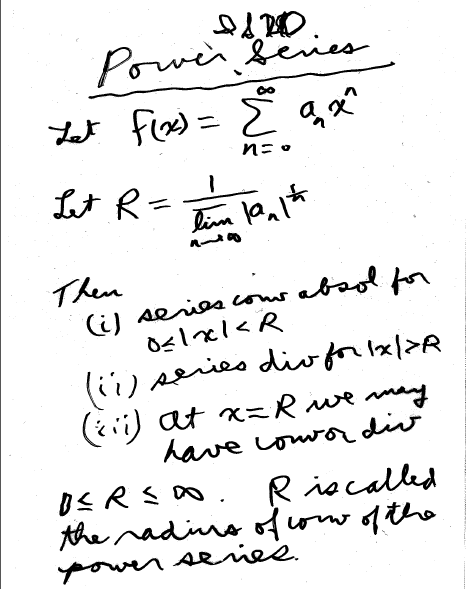
\includegraphics[scale=.7]{Pages/IS_20}

\end{center}

\newpage %21

\begin{center}

Infinite Series 21

\end{center}

{\underline {PF:}} By Root Test,

$\Sigma a_{n} x^{n} lone something$

if ${\underset{\text{$N\Rightarrow \infty$}}{\bar{lim}}}$ $|a_{n} x^{n}|^{\frac{1}{n}}<1$

if $|x|$ ${\underset{\text{$N\Rightarrow \infty$}}{\bar{lim}}}$ $|a_{n}|^{\frac{1}{n}}$

if $|x|$ $<$ ${\frac{1}{lim|a_{n}|}^{\frac{1}{n}}}$

if $|x|$ $lim n->\infty$ ${|a_{n}}|^{\frac{1}{n}}$

if $|x|$ $<$ ${\frac{1}{lim}}{|a_{n}}|^{\frac{1}{n}} = R$

If ${\bar{lim}}$ ${|a_{n}x^{n}}|{\frac{1}{n}} > 1$ soive div

And series div if $|x| > R$ 

When $|x| = R$ anything can happen
\begin{center}

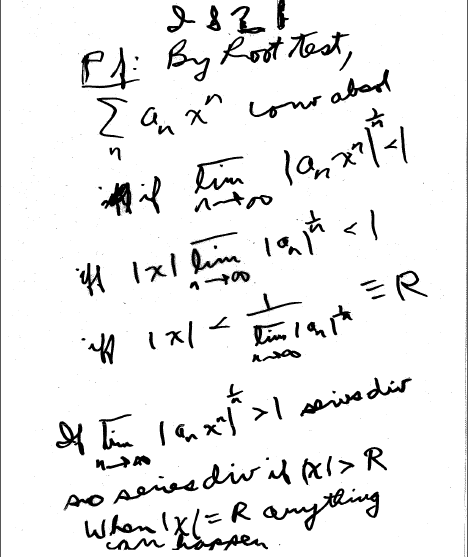
\includegraphics[scale=.7]{Pages/IS_21}

\end{center}
\newpage %22

\begin{center}

Infinite Series 22

For Series $\Sigma$ $a_{n} st.$ $a, \geq a_{z} \geq $ .. $\geq 0$ 

We can obtain two separate equal conditions chastening comes or div

{\underline {Thml}} (Cauchy Condoumsatism The)If $a_{1} \geq a_{2} \geq $ ... $\geq 0$ then

$\frac{1}{2}$ $\underset{\text{k=1}}{\overset{\text{$\infty$}}{\Sigma}}$ $\overset{\text{k}}{2a_{2k}}$ $\leq \underset{\text{n=1}}{\overset{\text{$\infty$}}{\Sigma}} {a_{n}}$ $\leq \underset{\text{k=0}}{\overset{\text{$\infty$}}{\Sigma}}$ $\overset{\text{k}}{2a_{2k}}$

ntense $\Sigma a_{n}$ and $\Sigma 2^{k}$ $a_{2k}$

consomething n divege something

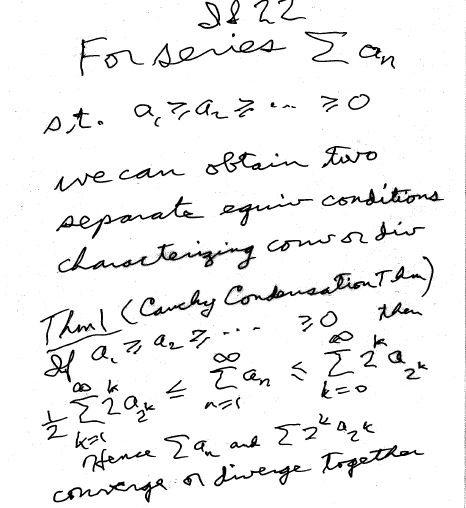
\includegraphics[scale=.7]{Pages/IS_22}

\end{center}

\newpage %23

\begin{center}

Infinite Series 23

\underline{Pfi} $\underset{\text{k=1}}{\overset{\text{$\infty$}}{\Sigma}}$ ${a_{k}}$ $= \underset{\text{$\infty$=0}}{\overset{\text{$\infty$}}{\Sigma}}$
$({\underset{\text{$2^{n}\leq k < 2^{n+s}$}}{\Sigma a_{k}}})$

$\frac{1}{2}(2^{n+1}a_{2n+1}) \leq {\underset{\text{$2^{n}\leq k < 2^{n+1}$}}{\Sigma a_{k}}}$ $\leq 2^{n}a_{2n}$

Summing over $n \geq 0$ given

$\frac{1}{2}\underset{\text{n=1}}{\overset{\text{$\infty$}}{\Sigma}} 2^{n}a_{2n} \leq \underset{\text{k=1}}{\overset{\text{$\infty$}}{\Sigma}} a_{k}$ $\underset{\text{n=0}}{\overset{\text{$\infty$}}{\Sigma}}2^{n}a_{2n}$

\end{center}

Application

\begin{center}

$\Sigma \frac{1}{n} = \infty$ $iH \underset{\text{n=0}}{\overset{\text{$\infty$}}{\Sigma}}a_{k}$ $\leq \underset{\text{n=0}}{\overset{\text{$\infty$}}{\Sigma}}$ $1=\infty$

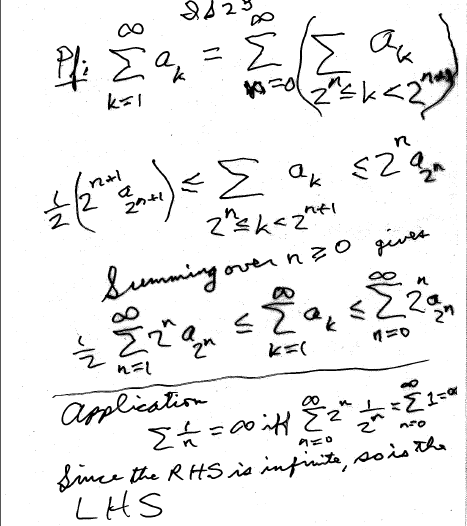
\includegraphics[scale=.7]{Pages/IS_23}

\end{center}

Since the RHS is infinite, so is the LHS

%Rebecca: IS24 - IS32

%Maady: IS33 - IS42

\section{Metric Spaces Part 1}

%Travis: M1 - M5

%Jerome: M6- M10



\section{Metric Spaces Part 2}


%Bryant: M1-M7

%Reshma: M8-M14

%Ethan: M15-M21




\end{document}